\documentclass[UTF8,a4paper,12pt]{ctexart}

\usepackage{geometry}
\usepackage{graphicx}
\usepackage{booktabs}
\usepackage{amsmath}
\usepackage{float}
\usepackage{caption}
\usepackage{subcaption}
\usepackage{hyperref}
\usepackage{xcolor}

\geometry{left=2.6cm,right=2.6cm,top=2.8cm,bottom=2.8cm}
\graphicspath{{figures/}{figures/progress_report/}}

\hypersetup{
  colorlinks=true,
  linkcolor=blue,
  citecolor=blue,
  urlcolor=blue
}

\newcommand{\pathtext}[1]{\texttt{\detokenize{#1}}}
\newcommand{\reportfig}[3][0.92\textwidth]{
  \begin{figure}[H]
    \centering
    \includegraphics[width=#1]{#2}
    \caption{#3}
  \end{figure}
}

\title{基于全景图预处理与传统算法候选挖掘的低空小目标检测数据构建进展报告}
\author{DMX 项目组}
\date{\today}

\begin{document}
\maketitle

\begin{abstract}
本文针对 DMX 全景图像采集与目标检测系统近期开发工作进行阶段总结。当前工作围绕低空小目标检测前处理展开，完成了 RGB/BW 原始图像读取、AB 半全景拼接、BW 图像旋转对齐、地平线分割、天空区域约束、传统图像处理疑似目标检测、256$\times$256 目标截图保存、640$\times$640 YOLOv26s 训练窗口挖掘，以及新雷达交互页面设计。系统当前目标是利用传统算法以高召回方式提取疑似目标区域，并将候选区域作为后续 YOLOv26s 训练和推理的数据基础。
\end{abstract}

\noindent\textbf{关键词：} 全景图像；地平线分割；传统目标检测；疑似目标挖掘；YOLOv26s；极坐标投影；雷达交互界面

\tableofcontents
\newpage

\section{阶段目标}

本阶段工作的核心目标是建立从全景原始图像到深度学习训练数据的完整前处理链路。整体思路为：先通过传统图像处理算法从天空区域中高召回提取疑似小目标，再将疑似目标截图和训练窗口组织为 YOLOv26s 的训练与推理数据基础。

\subsection{总体目标}

\begin{itemize}
  \item 建立 RGB/BW 图像读取、对齐、拼接与缩略显示流程。
  \item 利用开始阶段图像建立地平线背景，约束检测区域到天空区域。
  \item 使用传统算法提取疑似飞行物候选区域，并输出坐标、方位和截图。
  \item 形成候选目标截图目录规范，为后续人工筛选和模型训练提供数据。
  \item 构建 640$\times$640 训练窗口挖掘流程，服务 YOLOv26s 训练。
  \item 开发雷达式目标显示窗口，实现候选目标的时间列表、方位展示和图像交互。
\end{itemize}

\subsection{阶段技术路线}

\reportfig{stage_pipeline.png}{阶段技术路线图}

该路线将传统算法定位为候选挖掘器，而不是最终分类器。传统算法负责从大范围天空背景中快速发现疑似区域，并输出可追溯的坐标、截图和统计结果；YOLOv26s 负责在经过人工复核的数据集上学习小目标外观特征，后续再回到在线系统中进行推理和雷达页面显示。

\section{数据来源与图像组织}

\subsection{在线采集数据组织}

在线系统从设备端接收 RGB/BW 图像路径，读取共享盘图像后送入显示缓存、录制模块和候选检测模块。当前配置中，全景图宽度为 65536，高度为 4096；界面缩略条宽度为 8192，高度为 240。

\begin{table}[H]
  \centering
  \caption{当前全景与检测相关配置}
  \begin{tabular}{lll}
    \toprule
    配置项 & 当前值 & 说明 \\
    \midrule
    全景图宽度 & 65536 & 16 帧 4096 宽图像拼接 \\
    全景图高度 & 4096 & 当前设备帧高 \\
    缩略图宽度 & 8192 & UI 显示与雷达背景压缩使用 \\
    检测流 & BW & 当前优先使用黑白图降低误报与计算压力 \\
    背景建模帧数 & 3 & 开始阶段同位置前三张图像 \\
    候选截图尺寸 & 256$\times$256 & 传统算法疑似目标输出截图 \\
    YOLO 训练窗口 & 640$\times$640 & 训练样本挖掘窗口尺寸 \\
    \bottomrule
  \end{tabular}
\end{table}

\subsection{测试数据集 20161018-4}

本阶段传统算法测试使用样本目录：

\begin{center}
  \pathtext{/mnt/dmx4t/DMX_yangben/20161018-4}
\end{center}

该目录当前包含 1545 个文件，约 103 MB。图像为 256$\times$256 的 8 位 BMP 小图，文件名中包含采集通道、日期、时间以及疑似目标在全景坐标中的位置字段。样例文件名如下：

\begin{center}
  \pathtext{I9_20161018_093440_9177_2907.bmp}
\end{center}

其中可初步理解为：

\begin{itemize}
  \item \pathtext{I9}：数据通道或类别编号。
  \item \pathtext{20161018}：采集日期。
  \item \pathtext{093440}：采集时间。
  \item \pathtext{9177_2907}：疑似目标对应的原始全景坐标或裁剪中心坐标。
\end{itemize}

\begin{table}[H]
  \centering
  \caption{20161018-4 数据集文件前缀统计}
  \begin{tabular}{cc}
    \toprule
    文件前缀 & 数量 \\
    \midrule
    I1 & 116 \\
    I5 & 542 \\
    I9 & 886 \\
    \bottomrule
  \end{tabular}
\end{table}

\reportfig{dataset_20161018_samples.png}{20161018-4 样本图像缩略图矩阵}
\reportfig[0.72\textwidth]{dataset_20161018_prefix_counts.png}{20161018-4 数据前缀数量与传统算法检出数量统计}

\subsection{采集数据集 20260626}

除 20161018-4 历史小图样本外，当前还整理了 20260626 采集数据：

\begin{center}
  \pathtext{/mnt/dmx4t/DMX_yangben/20260626}
\end{center}

该目录下已包含按流类型、小时和样本类别组织的 candidate/negative 图像，可作为 YOLOv26s 联合训练数据来源。目录结构示例如下：

\begin{center}
  \pathtext{20260626/<bw|rgb>/<HH>/<candidate|negative>/图片}
\end{center}

\begin{table}[H]
  \centering
  \caption{20260626 采集数据样本统计}
  \begin{tabular}{lrrr}
    \toprule
    数据流 & candidate & negative & 合计 \\
    \midrule
    BW & 1180 & 1596 & 2776 \\
    RGB & 3520 & 2748 & 6268 \\
    \midrule
    合计 & 4700 & 4344 & 9044 \\
    \bottomrule
  \end{tabular}
\end{table}

20260626 数据与 20161018-4 的作用不同：20161018-4 主要用于验证传统算法在 256$\times$256 小目标裁剪图上的检出能力；20260626 则更接近当前系统采集流程，包含 BW/RGB、candidate/negative 和 640$\times$640 训练窗口样本。因此后续 YOLOv26s 训练应将两批数据合并使用，但需要在数据配置中保留来源字段，便于后续按数据来源分析误检和漏检。

\section{图像预处理流程}

\subsection{原始图读取与格式统一}

系统读取设备共享盘或本地样本目录中的图像文件后，将不同来源的图像统一转换为后续算法可处理的灰度图或 RGB32 图像。对于在线系统，RGB 和 BW 图像分别进入不同处理线程，并通过时间戳和角度回查机制完成角度关联。

\subsection{BW 图旋转对齐}

近期处理中确认 BW 图需要旋转 180 度后再与 RGB 图对齐。对齐后的 BW 图用于传统检测和雷达背景投影，可以减少 RGB/BW 画面方位不一致造成的目标定位误差。

\reportfig{bw_rotate180_alignment_compare.png}{BW 图旋转 180 度前后对比}

\subsection{AB 半全景拼接}

录制模块当前输出 AB 半全景 JPG，而不再保存大量原始单帧。保存路径规则为：

\begin{center}
  \pathtext{recordRoot/YYYYMMDD/<rgb|bw>/HH/原始名-A或B.jpg}
\end{center}

当前配置中的录制根目录为：

\begin{center}
  \pathtext{/mnt/dmx4t/data/recordings}
\end{center}

\reportfig{bw_pano_rot180_8192x512.jpg}{BW AB 半全景拼接与旋转对齐后的缩略图}

\section{地平线分割方法}

\subsection{物理含义}

地平线分割的目标不是只找一条几何直线，而是把全景图中草坪、道路、树篱、楼体等地面连接区域与天空区域分开。对于后续检测而言，真正需要的是天空检测 mask：目标检测只在地平线以上或地面 mask 之外的区域进行，从而减少草坪纹理、建筑边缘、树线和拼接边界带来的误检。

对于雷达背景极坐标投影，图像 $y$ 方向的物理含义定义为天空高度：越靠近图像上方表示越高的天空区域，越靠近地平线或地面表示越低的天空区域。因此地平线分割结果同时影响两个模块：一是传统小目标检测的候选区域约束，二是雷达极坐标背景中半径方向的物理解释。

\subsection{草坪/地面连通区域分割}

20260626 数据中已经生成了草坪分割和地平线分割可视化结果，位于：

\begin{center}
  \pathtext{/mnt/dmx4t/DMX_yangben/20260626/_analysis/horizon_preview_ground}
\end{center}

该方法以地面区域为主体进行分割，而不是简单依赖单行亮度差。主要流程如下：

\begin{enumerate}
  \item 对 BW 全景图灰度化并进行高斯平滑，降低草坪细纹理和图像噪声。
  \item 在图像下半部分估计地面亮度/纹理阈值，得到初始地面候选区域。
  \item 使用形态学闭运算连接草坪、道路等被纹理断开的区域。
  \item 使用形态学开运算去除小面积噪声点。
  \item 只保留与图像底部连通的大面积区域，得到 bottom-connected ground mask。
  \item 对每一列寻找地面 mask 的最上边界，形成地平线候选曲线。
  \item 对边界曲线进行中值滤波和平滑，得到稳定的地平线/草坪上边界。
\end{enumerate}

地面连通区域可表示为：

\[
  G = \operatorname{Conn}_{\mathrm{bottom}}\left(\operatorname{Open}\left(\operatorname{Close}(T(I))\right)\right)
\]

其中 $T(I)$ 表示阈值化后的初始地面候选，$\operatorname{Close}(\cdot)$ 用于连接断裂区域，$\operatorname{Open}(\cdot)$ 用于去除小噪声，$\operatorname{Conn}_{\mathrm{bottom}}(\cdot)$ 表示保留与图像底部连通的区域。

\subsection{地平线曲线与天空 mask}

对每一列 $x$，从上到下寻找地面 mask 的第一个像素位置，得到地面上边界：

\[
  h(x) = \min\{y \mid G(x,y)=1\}
\]

随后对 $h(x)$ 进行中值滤波：

\[
  \hat{h}(x)=\operatorname{median}\left(h(x-k),\ldots,h(x+k)\right)
\]

最终天空检测区域定义为：

\[
  S(x,y)=
  \begin{cases}
    1, & y < \hat{h}(x)-m \\
    0, & y \geq \hat{h}(x)-m
  \end{cases}
\]

其中 $m$ 为安全边距，当前配置中对应 \pathtext{skyMargin=16}。该边距用于把检测区域从地平线向上收缩，避免草坪边缘、树篱顶部和建筑边缘进入目标检测区域。

\subsection{可视化对比}

图 \ref{fig:ground-horizon-contact} 展示了多组 BW 全景图的草坪/地面分割和天空保留区域对比。每组结果中包含原始图、地面区域覆盖图和天空检测区域图，可以直接观察草坪分割是否覆盖了地面连接区域，以及天空区域是否保留完整。

\begin{figure}[H]
  \centering
  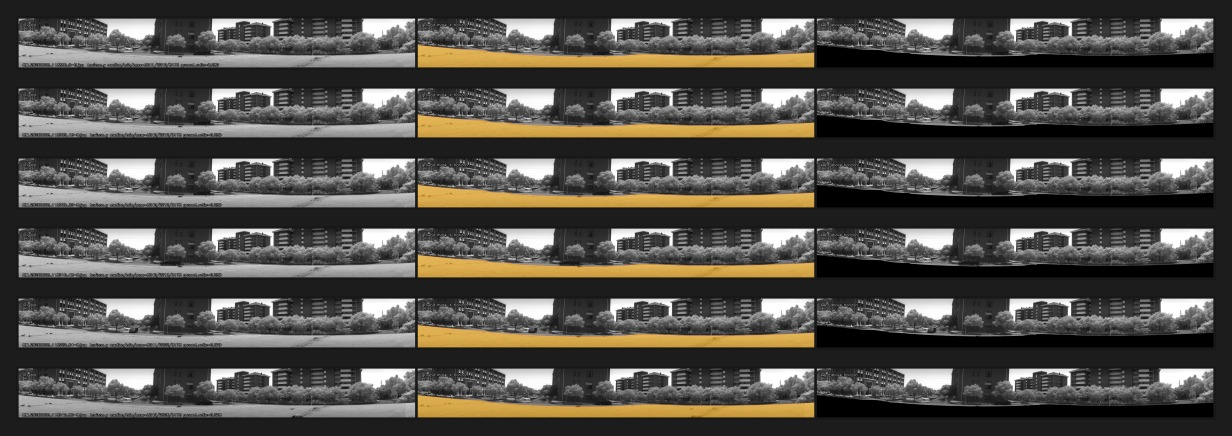
\includegraphics[width=0.96\textwidth]{ground_horizon_contact_sheet.jpg}
  \caption{20260626 草坪/地面分割与地平线区域对比}
  \label{fig:ground-horizon-contact}
\end{figure}

图 \ref{fig:skyline-contact} 展示了地平线曲线检测效果。该可视化用于观察曲线在建筑、树线、草坪和天空交界处的稳定性。

\begin{figure}[H]
  \centering
  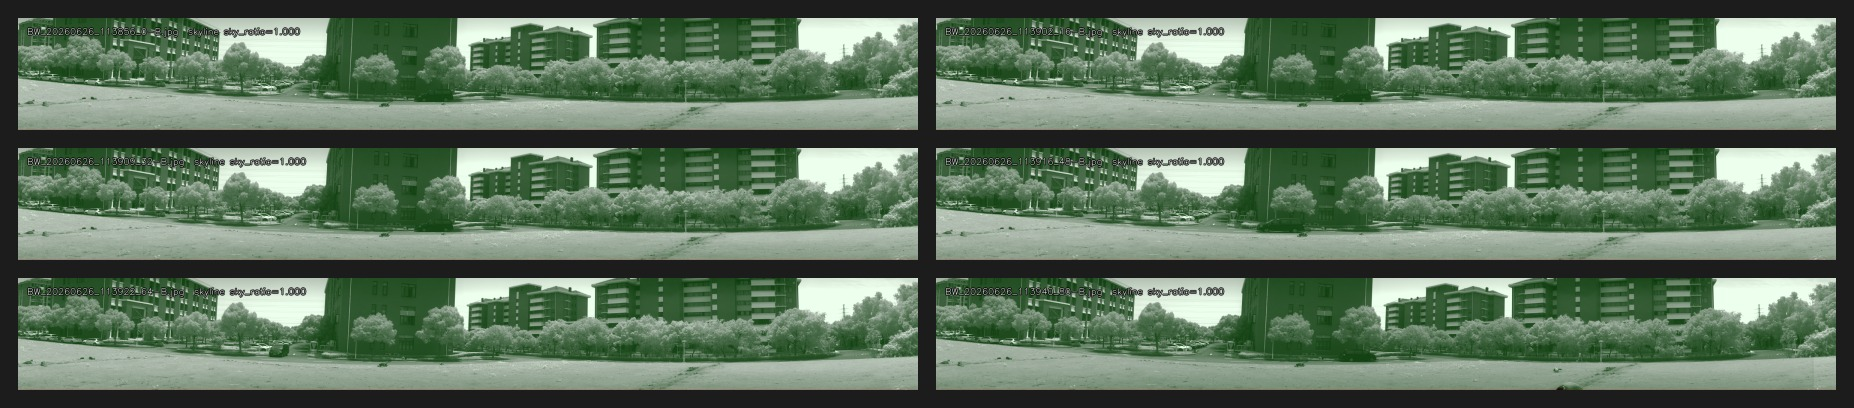
\includegraphics[width=0.96\textwidth]{skyline_preview_contact_sheet.jpg}
  \caption{20260626 地平线曲线检测对比}
  \label{fig:skyline-contact}
\end{figure}

单张全景的地面 mask 和地平线测试结果保存在：

\begin{center}
  \pathtext{/mnt/dmx4t/DMX_yangben/20260626/_analysis/horizon_test}
\end{center}

对应结果如图 \ref{fig:horizon-test-single} 所示。该图更适合查看单张图上的 mask 边界和分割细节。

\begin{figure}[H]
  \centering
  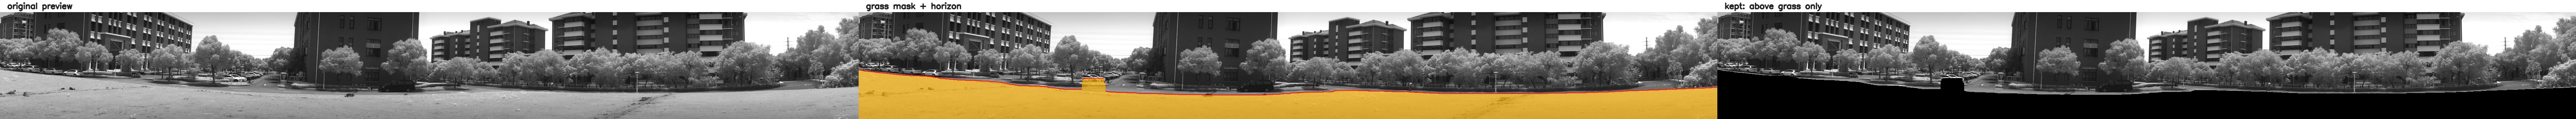
\includegraphics[width=0.92\textwidth]{horizon_test_single.jpg}
  \caption{单张 BW 全景地平线分割测试结果}
  \label{fig:horizon-test-single}
\end{figure}

\section{传统疑似目标检测算法}

\subsection{背景建模}

程序运行后，使用每个全景 tile 起始阶段的前三张图像建立背景：

\[
  B(x,y) = \frac{1}{N}\sum_{i=1}^{N} I_i(x,y), \quad N=3
\]

其中 $I_i(x,y)$ 表示第 $i$ 张输入图像在 $(x,y)$ 位置的灰度值，$B(x,y)$ 表示背景模型。

\subsection{背景差分}

当前帧与背景图做差，得到运动或异常响应：

\[
  D(x,y) = |I(x,y) - B(x,y)|
\]

\subsection{TopHat 小目标增强}

为了增强天空背景中的小亮目标，使用形态学 TopHat 操作：

\[
  R(x,y) = I(x,y) - \operatorname{open}(I)(x,y)
\]

其中 $\operatorname{open}(\cdot)$ 表示形态学开运算。当前配置中 TopHat 核大小为 15。

在 20161018-4 小图测试中，目标既可能表现为亮斑，也可能表现为暗色飞行物。因此测试脚本同时计算亮目标响应和暗目标响应：

\[
  R_{\mathrm{bright}} = I - \operatorname{open}(I)
\]

\[
  R_{\mathrm{dark}} = \operatorname{close}(I) - I
\]

\[
  R = \max(R_{\mathrm{bright}}, R_{\mathrm{dark}})
\]

其中 $\operatorname{close}(\cdot)$ 表示形态学闭运算。该处理可以同时覆盖天空中的亮点目标和暗色飞行物轮廓。

\subsection{自适应阈值}

候选二值图使用均值与标准差构造阈值：

\[
  T = \mu_D + k\sigma_D
\]

\[
  M(x,y) =
  \begin{cases}
    1, & D(x,y) > T \\
    0, & D(x,y) \leq T
  \end{cases}
\]

当前 $k=3.5$。随后对二值图进行连通域分析、面积过滤、局部对比度过滤和 NMS 去重。

\subsection{候选过滤与去重}

连通域过滤主要用于剔除过小噪声和过大背景结构。对每个连通域 $C_i$ 计算面积 $A_i$、中心点 $(x_i,y_i)$、局部对比度 $\Delta_i$ 和响应强度 $R_i$。候选得分可表示为：

\[
  S_i = R_i + 1.5\Delta_i + 0.25A_i
\]

候选按得分从高到低排序后执行非极大值抑制。若两个候选中心距离小于设定半径，则保留得分较高者：

\[
  \sqrt{(x_i-x_j)^2+(y_i-y_j)^2} > r_{\mathrm{nms}}
\]

在线系统中当前 NMS 半径为 96 像素；20161018-4 小图测试中由于图像只有 256$\times$256，使用了更小的局部去重半径。

\begin{table}[H]
  \centering
  \caption{传统候选检测参数}
  \begin{tabular}{lll}
    \toprule
    参数 & 当前值 & 作用 \\
    \midrule
    stream & BW & 检测图像流 \\
    backgroundFrames & 3 & 背景建模帧数 \\
    skyMargin & 16 & 地平线向上收缩边距 \\
    maxCandidatesPerFrame & 3 & 单帧最大候选数 \\
    minArea & 4 & 最小连通域面积 \\
    maxArea & 400 & 最大连通域面积 \\
    medianKernel & 3 & 中值滤波核 \\
    tophatKernel & 15 & 小目标增强核 \\
    thresholdK & 3.5 & 自适应阈值系数 \\
    minContrast & 25 & 最小局部对比度 \\
    nmsRadius & 96 & 去重半径 \\
    jpegQuality & 95 & 候选截图 JPEG 质量 \\
    \bottomrule
  \end{tabular}
\end{table}

\reportfig{traditional_detection_pipeline.png}{传统检测中间结果对比}

\section{疑似目标截图存储规范}

\subsection{截图尺寸与保存根路径}

当前传统算法输出疑似目标截图尺寸为 256$\times$256。保存根路径写在配置参数中：

\begin{center}
  \pathtext{/mnt/dmx4t/data/candidates}
\end{center}

目录层级建议在报告中统一描述为：

\begin{center}
  \pathtext{saveRoot/YYYYMMDD/HH/候选目标图片}
\end{center}

同时输出 \pathtext{manifest.jsonl} 记录目标时间、流类型、方位角、全景坐标、候选得分和截图路径。

\subsection{保存路径示例}

当前候选截图保存路径示例如下：

\begin{center}
  \pathtext{/mnt/dmx4t/data/candidates/20260626/11/}\\
  \pathtext{BW_20260626_113856_000001_x06224_y01736.jpg}
\end{center}

\reportfig{traditional_detection_top.png}{20161018-4 高响应疑似目标检出样例}

\section{面向 YOLOv26s 的训练样本窗口挖掘}

\subsection{传统算法作为高召回候选挖掘器}

当前策略不是直接让深度模型从全景图中盲检，而是先利用传统算法从天空区域中提取疑似目标候选，再将候选窗口、负样本窗口和可视化结果组织为训练数据。这样可以降低人工筛选成本，并提升小目标样本积累效率。

\subsection{训练窗口配置}

训练窗口挖掘脚本当前以 640$\times$640 为基本窗口，步长为 512。窗口得分综合小目标响应、连通域数量、边缘密度、纹理强度和地面占比等指标。

\[
  S = 0.36R_{\max} + 14C_{\mathrm{iso}} + 0.16\bar{R} - P_{\mathrm{texture}}
\]

其中 $R_{\max}$ 为窗口内最大响应，$C_{\mathrm{iso}}$ 为孤立目标得分，$\bar{R}$ 为平均响应，$P_{\mathrm{texture}}$ 为纹理惩罚项。

\begin{table}[H]
  \centering
  \caption{YOLOv26s 训练窗口挖掘配置}
  \begin{tabular}{lll}
    \toprule
    参数 & 当前值 & 说明 \\
    \midrule
    tile & 640 & 训练窗口尺寸 \\
    stride & 512 & 滑窗步长 \\
    maxCandidates & 8 & 单张源图最大候选窗口数 \\
    negative & 可配置 & 负样本窗口数量 \\
    maxGroundRatio & 0.12 & 候选窗口最大地面占比 \\
    输出类别 & candidate/negative & 候选样本与负样本 \\
    \bottomrule
  \end{tabular}
\end{table}

\subsection{20161018-4 原生尺寸初始训练集导出}

针对 20161018-4 历史样本，已将传统算法检出的疑似目标整理为 YOLOv26s 初始训练集。该批数据本身是 256$\times$256 裁剪小图，因此当前导出版本保持原生 256$\times$256 尺寸，不做 640 画布填充。这样可以避免引入人工灰色边界、中心区域偏置和目标相对尺度变化。后续训练时建议使用 \pathtext{imgsz=256} 或 \pathtext{imgsz=320} 做初步验证；真正的 640$\times$640 训练窗口应从原始全景图中按坐标回裁生成。

导出路径为：

\begin{center}
  \pathtext{latex/data/progress_report/yolo26s_seed_20161018_native256}
\end{center}

目录结构如下：

\begin{center}
\begin{tabular}{ll}
  \toprule
  路径 & 内容 \\
  \midrule
  \pathtext{images/train} & 训练图像 \\
  \pathtext{images/val} & 验证图像 \\
  \pathtext{labels/train} & 训练标签 \\
  \pathtext{labels/val} & 验证标签 \\
  \pathtext{data.yaml} & YOLO 数据集配置 \\
  \pathtext{manifest.csv} & 样本来源与伪标注记录 \\
  \pathtext{summary.csv} & 训练/验证统计 \\
  \bottomrule
\end{tabular}
\end{center}

\begin{table}[H]
  \centering
  \caption{YOLOv26s 初始训练集统计}
  \begin{tabular}{lrrrr}
    \toprule
    数据划分 & 图像数 & 正样本图像 & 负样本图像 & 标注框数 \\
    \midrule
    train & 1134 & 567 & 567 & 1281 \\
    val & 284 & 142 & 142 & 285 \\
    \midrule
    合计 & 1418 & 709 & 709 & 1566 \\
    \bottomrule
  \end{tabular}
\end{table}

\reportfig{yolo26s_seed_native256_samples.png}{YOLOv26s 原生 256$\times$256 初始训练集正样本与传统算法伪标注框}

需要注意的是，当前标签来自传统算法自动生成，属于伪标注。后续正式训练前应进行人工复核，删除云层纹理、边框、噪声等误检框，并补充传统算法未检出的低对比度目标。

此前测试过 640$\times$640 填充版导出流程，该版本仅适合验证 YOLO 目录结构和标签格式，不建议作为正式训练集使用。正式 640$\times$640 数据应从原始全景图按目标坐标回裁，保证图像上下文和目标尺度来自真实采集场景。

\subsection{联合训练数据组织策略}

后续训练建议将 20161018-4 与 20260626 两批数据合并，但不直接混成不可追踪的单一目录。推荐统一导出为如下结构：

\begin{center}
\begin{tabular}{ll}
  \toprule
  子目录 & 数据来源 \\
  \midrule
  \pathtext{images/train}、\pathtext{labels/train} & 训练图像与标签 \\
  \pathtext{images/val}、\pathtext{labels/val} & 验证图像与标签 \\
  \pathtext{manifest.csv} & 每张图像的来源、流类型、时间、样本类别 \\
  \pathtext{data.yaml} & YOLOv26s 数据集配置 \\
  \bottomrule
\end{tabular}
\end{center}

联合训练时建议采用两阶段策略：

\begin{enumerate}
  \item 第一阶段使用 20161018-4 原生 256$\times$256 数据快速验证小目标学习能力。
  \item 第二阶段加入 20260626 的 640$\times$640 candidate/negative 窗口，训练接近当前系统采集场景的模型。
  \item 第三阶段根据模型误检情况回到 20260626 中补充困难负样本，例如云层纹理、地面边缘、拼接边界和亮斑噪声。
\end{enumerate}

由于两批数据分辨率和上下文不同，训练时需要注意输入尺寸设置。20161018-4 适合 \pathtext{imgsz=256} 或 \pathtext{imgsz=320}；20260626 的窗口样本适合 \pathtext{imgsz=640}。如果直接联合训练，可先统一重采样到同一输入尺寸，并在结果分析中分别统计两批数据的表现。

\subsection{伪标注人工复核规则}

当前初始训练集来自传统算法自动候选，不能直接等同于人工真值。人工复核时建议采用以下规则：

\begin{enumerate}
  \item 保留具有明确飞行物轮廓、点状目标或连续运动轨迹依据的候选框。
  \item 删除云层纹理、压缩噪声、底部边框、树线、建筑边缘等误检框。
  \item 对明显框偏移的样本，重新调整框中心和大小，使目标主体完全落入框内。
  \item 对同一图像内多个候选目标，保留真实目标，删除背景结构重复框。
  \item 对传统算法未检出的明显目标，补充人工框，作为低对比度困难正样本。
  \item 保留一部分容易误检的背景图作为困难负样本，增强模型区分能力。
\end{enumerate}

\subsection{训练使用建议}

原生 256$\times$256 数据集适合做第一轮快速验证，建议训练入口使用较小输入尺寸，例如：

\begin{center}
  \pathtext{imgsz=256} 或 \pathtext{imgsz=320}
\end{center}

如果后续从原始全景图中回裁 640$\times$640 训练窗口，则再切换到 \pathtext{imgsz=640}。这样可以避免当前历史小图被强行填充带来的尺度偏差。

\section{Block2All 图片合并脚本}

\subsection{脚本目标}

Block2All 用于将原始分块图像或录制会话数据合并为 AB 半全景 JPG。脚本支持命令行模式和 Tkinter 图形界面，便于批处理历史数据和人工选择目录。

\subsection{核心处理逻辑}

\begin{enumerate}
  \item 自动识别输入路径是录制会话、日期目录还是原始数据树。
  \item 按 RGB/BW 流分别读取图像。
  \item 按文件编号或时间排序。
  \item 每 \pathtext{halfCount} 张图像组成一个半全景。
  \item 每帧先逆时针旋转 90 度再水平镜像。
  \item 半全景内部按序号逆序拼接。
  \item 输出 JPG，质量为 95。
  \item 生成 manifest JSON，记录输入、输出、跳过、失败和尾帧丢弃信息。
\end{enumerate}

\subsection{图形界面}

图形界面包含原始数据路径、目的路径、每半全景图像帧数、要生成全景图数量、处理流选择和运行日志区域。

\reportfig[0.82\textwidth]{block2all_gui_schematic.png}{Block2All 图形界面与参数配置}

\subsection{命令行使用方式}

脚本无参数启动时进入图形界面；带参数时可直接批处理。例如处理原始数据树并每 8 帧生成一个半全景：

\begin{center}
  \pathtext{python3 tools/block2all.py SRC_DIR OUT_ROOT 8}
\end{center}

若只处理 BW 流，可使用：

\begin{center}
  \pathtext{python3 tools/block2all.py SRC_DIR OUT_ROOT 8 --stream BW}
\end{center}

输出 manifest 中会记录处理模式、输入帧数、输出图像数、跳过数量、失败组数量、尾帧丢弃数量、方向变换规则和拼接顺序。

\section{新雷达窗口控件}

\subsection{页面布局}

新雷达页面按照 1920$\times$1080 和 3840$\times$2160 屏幕设计，采用三栏布局：

\begin{itemize}
  \item 左侧：目标图像列表，按目标出现时间动态更新。
  \item 中间：雷达极坐标图，显示网格、扫描角、背景全景投影和目标点。
  \item 右侧上半部分：目标信息面板，显示方位、坐标、得分、状态等。
  \item 右侧下半部分：目标位置图和交互预览图。
\end{itemize}

\reportfig{radar_ui_mock_1920x1080.jpg}{新雷达页面 1920$\times$1080 整体布局}

页面切换逻辑采用主界面页面栈切换方式，而不是将新控件覆盖到旧页面上。这样可以避免旧页面残留、文字框重叠和控件互相遮挡。右侧预览区域采用固定布局尺寸，目标切换时只更新图像内容，避免交互图像在切换后缓慢缩放。

\subsection{控件工程结构}

新页面控件被放置在 \pathtext{radar_ui} 子目录下，主要模块包括：

\begin{table}[H]
  \centering
  \caption{雷达页面控件结构}
  \begin{tabular}{ll}
    \toprule
    文件/控件 & 功能 \\
    \midrule
    \pathtext{targetradarwindow} & 雷达页面总容器与测试入口 \\
    \pathtext{targetradarwidget} & 中间雷达图绘制与点击交互 \\
    \pathtext{targetlistwidget} & 左侧目标列表 \\
    \pathtext{targetinfopanel} & 右侧目标信息面板 \\
    \pathtext{targetpreviewpanel} & 右下目标图像预览 \\
    \pathtext{polarpanoramaprojector} & 全景图极坐标投影 \\
    \pathtext{targetrecord} & 目标数据结构 \\
    \bottomrule
  \end{tabular}
\end{table}

\section{极坐标背景投影方法}

\subsection{横轴到方位角映射}

全景图横轴 $x$ 表示 0 到 360 度方位：

\[
  \theta = 2\pi \frac{x}{W}
\]

其中 $W$ 为全景图宽度。

\subsection{纵轴到天空高度半径映射}

图像 $y$ 方向被定义为天空高度，越靠近图像上方代表越高天空，投影到雷达图时越靠外圈；越靠近地平线或地面，投影越靠内圈：

\[
  r = R_{\mathrm{inner}} + \left(1 - \frac{y}{H}\right)(R_{\mathrm{outer}} - R_{\mathrm{inner}})
\]

\subsection{极坐标到屏幕坐标}

雷达图中以正北方向为 0 度，顺时针为正方向：

\[
  X = C_x + r\sin\theta
\]

\[
  Y = C_y - r\cos\theta
\]

其中 $(C_x,C_y)$ 为雷达图中心点。

\reportfig{panorama_to_polar_compare.png}{全景图到雷达极坐标背景的投影效果}

当前投影示例使用 BW 全景背景，并已完成 180 度方位对齐。后续融合模式可以在同一极坐标映射框架下将 RGB、BW 或融合图作为输入背景，只需要保证不同源图像在方位轴上完成对齐。

\section{20161018-4 数据传统算法测试计划}

\subsection{测试目标}

该批数据包含小物体飞行物样本和天空背景样本，适合用于验证传统算法在小尺寸图像上的候选提取能力。样本图像尺寸为 256$\times$256。测试目标包括：

\begin{itemize}
  \item 统计候选检出数量与不同前缀数据的响应差异。
  \item 可视化传统算法中间结果。
  \item 分析云层、噪声、边缘纹理造成的误检。
  \item 按文件名中的坐标字段回写候选来源位置。
  \item 筛选可用于 YOLOv26s 初始训练的正样本和困难负样本。
\end{itemize}

\subsection{计划输出}

\begin{table}[H]
  \centering
  \caption{20161018-4 传统算法测试计划输出}
  \begin{tabular}{lll}
    \toprule
    输出内容 & 保存位置 & 用途 \\
    \midrule
    样本缩略图矩阵 & \pathtext{latex/figures/progress_report} & 报告可视化 \\
    检测中间图 & \pathtext{latex/figures/progress_report} & 展示算法流程 \\
    候选框结果图 & \pathtext{latex/figures/progress_report} & 展示识别效果 \\
    候选统计 CSV & \pathtext{latex/data/progress_report} & 数据分析 \\
    目标/背景对比图 & \pathtext{latex/figures/progress_report} & 说明误检与漏检 \\
    \bottomrule
  \end{tabular}
\end{table}

\subsection{初步测试结果}

已对 \pathtext{/mnt/dmx4t/DMX_yangben/20161018-4} 中的 1544 张 BMP 图像进行传统算法初步测试。测试算法同时增强亮目标和暗目标响应，并屏蔽图像底部边框伪响应。当前结果以候选挖掘为目标，优先保证疑似目标召回，后续再通过人工复核和 YOLOv26s 训练降低误检。

\begin{table}[H]
  \centering
  \caption{20161018-4 传统算法初步测试统计}
  \begin{tabular}{lrrrr}
    \toprule
    数据前缀 & 样本数 & 检出样本数 & 检出率 & 说明 \\
    \midrule
    I1 & 116 & 62 & 53.4\% & 小目标响应较明显 \\
    I5 & 542 & 145 & 26.8\% & 低响应或背景类样本占比较高 \\
    I9 & 886 & 502 & 56.7\% & 检出样本数量最多 \\
    \midrule
    合计 & 1544 & 709 & 45.9\% & 共输出候选 1566 个 \\
    \bottomrule
  \end{tabular}
\end{table}

\reportfig[0.76\textwidth]{traditional_score_distribution.png}{传统算法最佳候选得分分布}
\reportfig[0.66\textwidth]{traditional_candidate_centers.png}{检出候选在 256$\times$256 裁剪图中的中心位置分布}
\reportfig{traditional_detection_low_response.png}{低响应或背景类样本示例}

从初步结果看，I9 与 I1 样本的候选检出率明显高于 I5。该现象说明不同前缀数据中小目标形态、对比度和背景纹理存在差异。后续将结合人工复核，将高响应候选作为正样本来源，将低响应背景、云层纹理和边缘干扰作为困难负样本来源，用于 YOLOv26s 训练。

\section{当前阶段成果}

\begin{itemize}
  \item 已完成配置化传统检测参数，包括检测流、背景帧数、TopHat 核、阈值系数、面积过滤、对比度过滤和 NMS。
  \item 已完成 256$\times$256 疑似目标截图存储逻辑，并通过配置指定保存根路径。
  \item 已完成 Block2All 图片合并脚本，支持命令行与图形界面。
  \item 已完成雷达页面控件初版，包括目标列表、雷达图、信息面板、预览面板和极坐标背景投影。
  \item 已明确 BW 图需旋转 180 度后与 RGB 对齐。
  \item 已建立面向 YOLOv26s 的 640$\times$640 训练窗口挖掘脚本。
  \item 已完成 20161018-4 历史样本传统算法测试，并生成统计图、候选图和中间过程图。
  \item 已导出 YOLOv26s 原生 256$\times$256 初始训练集，包含 train/val 划分、YOLO 标签、manifest 和 data.yaml。
\end{itemize}

\section{问题分析与下一阶段计划}

\subsection{当前问题}

\begin{itemize}
  \item 传统算法需要在更多历史数据上验证误检率与漏检情况。
  \item 云层纹理、树线、建筑边缘可能产生高响应，需要通过困难负样本进入 YOLOv26s 训练。
  \item 雷达页面背景投影还需要继续验证 BW/RGB/融合三种模式的视觉稳定性。
  \item 目标截图目录、manifest 字段和 YOLO 数据集格式需要进一步统一。
  \item 当前 20161018-4 数据集标签为传统算法伪标注，正式训练前必须人工复核。
  \item 历史 256$\times$256 小图缺少完整全景上下文，不能完全替代真实 640$\times$640 全景回裁窗口。
\end{itemize}

\subsection{下一阶段计划}

\begin{enumerate}
  \item 对 20161018-4 原生 256$\times$256 初始训练集进行人工复核，形成第一版 clean labels。
  \item 使用 \pathtext{imgsz=256} 或 \pathtext{imgsz=320} 训练 YOLOv26s 快速验证模型，观察误检与漏检类型。
  \item 根据模型误检结果补充困难负样本，根据漏检结果补充低对比度正样本。
  \item 基于原始全景图和文件名坐标字段，回裁真实 640$\times$640 训练窗口。
  \item 建立 YOLOv26s 推理输出到在线系统候选记录的接口，统一字段包括方位角、全景坐标、得分、截图路径。
  \item 将 YOLOv26s 推理结果接入新雷达页面，实现目标点、目标列表和右侧预览联动。
\end{enumerate}

\section{可复现实验命令}

\subsection{传统算法测试}

20161018-4 数据测试命令如下：

\begin{center}
  \pathtext{python3 tools/evaluate_traditional_20161018.py}
\end{center}

该命令输出：

\begin{itemize}
  \item \pathtext{latex/data/progress_report/traditional_20161018_results.csv}
  \item \pathtext{latex/data/progress_report/traditional_20161018_summary.csv}
  \item \pathtext{latex/figures/progress_report/traditional_detection_pipeline.png}
  \item \pathtext{latex/figures/progress_report/traditional_detection_top.png}
  \item \pathtext{latex/figures/progress_report/traditional_score_distribution.png}
\end{itemize}

\subsection{YOLOv26s 初始训练集导出}

原生 256$\times$256 数据集导出命令如下：

\begin{center}
  \pathtext{python3 tools/export_yolo26s_seed_20161018.py}
\end{center}

输出目录为：

\begin{center}
  \pathtext{latex/data/progress_report/yolo26s_seed_20161018_native256}
\end{center}

如果仅需验证 640$\times$640 YOLO 目录和标签格式，可临时执行：

\begin{center}
  \pathtext{python3 tools/export_yolo26s_seed_20161018.py --image-size 640}
\end{center}

该 640 填充版不建议作为正式训练数据。

\subsection{报告编译}

本文档使用 XeLaTeX 编译：

\begin{center}
  \pathtext{cd /home/sht/work/DMX_qt/latex}\\
  \pathtext{./build_progress.sh}
\end{center}

\end{document}
